\chapter{Radiative Transfer}
\label{cha:radiative-transfer}

\section{Introduction}
\label{sec:introduction}

We are going to set the stage for a deeper look at astrophysical
sources of radiation by defining the important concepts of radiative
transfer, thermal radiation and radiative diffusion.

One can make a large amount of progress by realizing that the
distances that radiation typically travels between emission and
detection or scattering etc. are much longer than the wavelength of
the radiation.  In this regime we can assume that light travels in
straight lines (called rays).  Upon these assumptions the field of
radiative transfer is built.

\section{Flux}
\label{sec:flux}
\index{radiation!flux}
Let's start with something familiar and give it a precise definition.
The flux is simply the rate that energy passes through an
infinitesimal area (imagine a small window).
\begin{equation}
dE = F d\!A dt
\label{eq:1}
\end{equation}
For example, if you have an isotropic source, 
the flux is constant across a spherical surface centered on the
source, so you find that
\begin{equation}
E_1=F_1 4 \pi R_1^2 ~\mbox{\rm and}~
E_2=F_2 4 \pi R_2^2 
\label{eq:2}
\end{equation}
at two radii around the source.   Unless there is aborption or scattering 
between the two radii, $E_1=E_2$ and we obtain the inverse-square law 
for flux
\begin{equation}
F_1 R_1^2 = F_2 R_2^2.
\label{eq:3}
\end{equation}

\begin{figure}
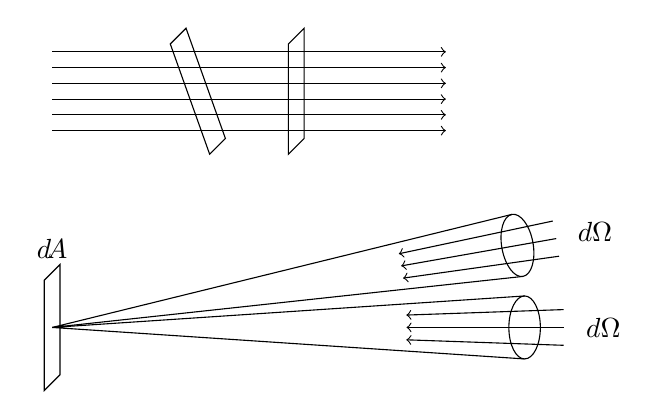
\begin{tikzpicture}
\begin{scope}[shift={(-6,-3)}]
\foreach \alpha in {0,10}  {
\begin{scope}[shift={(6,0)},rotate=\alpha]
\draw (6,0) ellipse (0.2 and 0.4);
\draw (6,0.4) -- (0,0) -- (6,-0.4);
\draw (7,0) node {$d \Omega$};
\foreach \ang in {-2,0,2} {
\draw [<-] (0,0) ++(\ang:4.5) -- ++(\ang:2);
}
\end{scope}
}
\draw (5.9,-0.8) -- (6.1,-0.6) -- (6.1,0.8) -- (5.9,0.6)  -- cycle ;
\draw (6,1) node {$d\!A$} ;
\end{scope}
\foreach \y in {-0.5,-0.3,...,0.5}  
{
\draw [->] (0,\y) -- (5,\y);
}
\draw (3,-0.8) -- (3.2,-0.6) -- (3.2,0.8) -- (3,0.6)  -- cycle ;
\draw (2,-0.8) -- (2.2,-0.6) -- (1.7,0.8) -- (1.5,0.6)  -- cycle ;

\end{tikzpicture}
\caption{Flux and intensity.  On the left the power delivered to the
  two surfaces are equal even though their areas differ.  The flux is
  the power per unit area so the tilted surface gets less flux.  On
  the right intensity is the power delivered to an area from a
  particular part of the sky (solid angle).  Here the two intensities
  are equal but the upper set of rays delivers less flux.}
\end{figure}
\section{Intensity}
\label{sec:intensity}
\index{radiation!intensity}

Although the flux is a useful quantity, it cannot encapsulate all of
our knowledge about a radiation field.  For example, one could shine a
faint light directly through a window or a bright light through the
same surface at an angle.  Both of these sitautions are characterized
by the same rate of energy flow through the surface, but they are
clearly different physical situations.

A more generally useful quantity quantifies the rate that energy flows
through a surface in a particular direction (imagine that the window
now looks into a long pipe so that only light travelling in a
particular direction can pass through,
\begin{equation}
dE = I d\!A d \Omega dt 
\label{eq:4}
\end{equation}
where $I$ is the intensity. Although this quantity seems a bit kludgy,
it is actually quite familiar.  It is the brightness.

You look at a light bulb.   As you move away from the light bulb, your
eye receives less flux ($F$ decreases) and the apparent size of the
light bulb also decreases ($d\Omega$ decreases).  It turns out that
these two quantities both decrease as $R^{-2}$, so the intensity or
brightness is conserved along a ray.  This result makes the intensity
a terrifically useful quantity.

\subsection{Relation to the flux}
\label{sec:relation-flux}

From the example at the beginning of this section we can deduce the 
relationship between the flux and the intensity of the light.
Radiation that travels perpendicular to a surface delivers more energy to 
that surface than radiation travelling at an angle.   You can always
imagine second surface perpendicular to the light ray through which all of
the energy that reaches the first surface travels.  We know that
intensity is the same along the ray so
\begin{equation}
d E = I d\!A_1 d \Omega d t= I d\!A_2 d \Omega d t
\label{eq:5}
\end{equation}
and $d\!A_2 = \cos \theta d\!A_1$, so the total flux travelling through
the surface is given by a moment of the intensity
\begin{equation}
F = \int I \cos \theta d \Omega
\label{eq:6}
\end{equation}
If $I$ is constant with respect to angle, there is as much energy
travelling from left to right as from right to left, so the net flux
vanishes, or more mathematically the mean of $\cos \theta$ vanishes 
over the sphere.

\paragraph{Something to think about}   The Sun is equally intense in
the summer and winter (if you exclude the effects of the
atmosphere), then why are winters colder than summers?   

A closely related quantity is the pressure that a radiation field
exerts on a surface.  Pressure is the rate that momentum is delivered 
to a surface in the direction perpendicular to the surface.  The
momentum of light is $E/c$ and the rate that energy is 
delivered to a surface from light travelling around a particular
direction is simply $I \cos \theta d\Omega$.  The component 
of the momentum that is directed perpendicular to the surface 
is $E \cos\theta/c$, so there is a second factor of $\cos \theta$ 
yielding the following integral.
\begin{equation}
p = \frac{1}{c} \int I \cos^2 \theta d \Omega.
\label{eq:7}
\end{equation}

\paragraph{Something to think about}  Does the radiation pressure 
from an isotropic radiation field vanish?

\subsection{Spectra}
\label{sec:spectra}

The quantities that we have defined so far can be examined as a
function of the frequency or wavelength of the radiation or the energy
of the individual photons, yielding $F_\nu, F_E, F_\lambda$ and 
also for the intensity, {\em e.g}
\begin{equation}
d E = F_{\nu} d \nu d\!A d t
\label{eq:8}
\end{equation}
and $F_\nu$ is called the specific flux.
The use of $F_{\nu}$ is so common that astronomers have a special 
unit to measure $F_\nu$
\begin{equation}
1~\hbox{\rm Jansky} = 1~\hbox{\rm Jy} = 10^{-26} \hbox{W m}^{-2}
\hbox{Hz}^{-1} = 10^{-23} \hbox{\rm erg cm}^{-1} \hbox{s}^{-1} \hbox{Hz}^{-1}.
\label{eq:9}
\end{equation}
This unit is most commonly used in the radio and infrared, and sometimes
in the x-rays.

A common combination that people use is 
\begin{equation}
E F_E = \lambda F_\lambda = \nu F_\nu  = \nu \frac{d F}{d \nu} =
\frac{d F}{d \ln \nu}.
\label{eq:10}
\end{equation}
This allows you to convert between $F_\nu$ and $F_\lambda$ etc.  And
it also gives the flux per logarithmic interval in photon energy or
frequency.  This is really handy since astronomers like to use log-log
plots.   A spectrum that goes as $F_\nu \propto 1/\nu$ has a constant 
amount of energy per logarithmic interval.

\paragraph{Something to think about}
A source emits at 1 Jansky from 100~MHz to 1~GHz and at 1 $\mu$Jy from
1 to 10 keV.  Is it brighter in the radio or x-rays?

\subsection{An Astronomical Aside: Magnitudes}
\label{sec:an-astr-asid}
\index{radiation!magnitudes}

Astronomers typically speak about the flux of an object in terms of 
magnitudes.   A magnitude is generally defined as
\begin{equation}
m = -2.5 \log_{10} \int_0^\infty g(\nu) F_{\nu,\Omega} d \nu + m_0.
\label{eq:11}
\end{equation}
What are the different quantities in this expression?  Pogson
empirically determined the value of ``2.5'' by comparing the
magnitudes of prominent observers of the 1800's.   It is remarkably close
to $\ln 10 \approx 2.3$, so a change in magnitude of 0.1 is about a 
ten-percent change in flux.

Another term in the expression is $g(\nu)$, the filter function that
determines which part of the electromagnetic spectrum you're are
looking at.  If $g(\nu)=1$, the quantity is called a ``bolometric
magnitude.''\index{radiation!bolometric magnitude}\index{bolometric
  magnitude}.  It is supposed to quantify the total energy coming from
the source.  One also hears about a quantity called the ``bolometric
correction''\index{bolometric correction} which is simply the
difference between the magnitude of source for a particular filter
($g(\nu)$) and for $g(\nu)=1$.

$F(\nu,\Omega)$ is the flux coming from the source as a function of
frequency integrated over a certain area of sky, $\Omega$.  For a star
one generally can extrapolate the flux that one observes in the sky to
the total flux, but the intensity from a galaxy or other extended
source generally falls off gradually so one defines a magnitude within
a certain aperture or down to a limiting intensity (surface
brightness).   

The final term is $m_0$, the zero point.  The value of the zero point
is a matter of convention.  Two of the standard conventions are the
``Vega'' convention which states that the magnitude of the star Vega
regardless of the function $g(\nu)$ is zero; all of Vega's colours are
zero.  This works nicely because you could always in principle observe
Vega with your equipment.

There are two problems however.  One is that the flux from Vega like
that of most stars varies a bit.  The second is that an object with a
flat spectrum (equal energies in each frequency interval) will have an
awkward set of colours (the difference in magnitudes for two different
$g(\nu)$ functions).  This leads to the second convention, the AB
system.
\begin{equation}
m(AB) = -2.5 \log_{10} f_\nu - 48.60 = -2.5 \log_{10} \left (
\frac{f_\nu}{1~\hbox{\rm Jy}}\right ) + 8.90
\label{eq:12}
\end{equation}
where $f_\nu$ is the flux in c.g.s. units.  The constants ``8.90'' 
and ``-48.60'' mean that $m(AB)=V$ for a flat spectrum source.

\paragraph{Something to think about}
How do you define an AB magnitude using a filter?

A final quantity that astronomers talk about is the surface
brightness.  This is just the intensity that we have been speaking
about all along.  However, the conventional nomenclature is rather strange,
magnitudes per square arcsecond.

\paragraph{Something to think about}
What is the magnitude of a source that subtends 10 square arcseconds
with a surface brightness of 19 magnitudes per square arcsecond?

\section{Energy Density}
\label{sec:energy-density}
\index{radiation!energy density}
Let's imagine that light is travelling through a small box.  How much
energy is in the box at any time?  First it is easiest to think about
how much energy in the box is travelling in a particular direction
through the box during a small time interval such that $c dt$ is the
length of the box,
\begin{equation}
d E = u(\Omega) d\!A c d t d\Omega
\label{eq:13}
\end{equation}
This energy equals the energy that enters the box travelling in the 
right direction during the time interval $dt$,
\begin{equation}
d E = I d\!A d t d\Omega
\label{eq:14}
\end{equation}
so
\begin{equation}
c u(\Omega) = I.
\label{eq:15}
\end{equation}
To get the total energy density you have to integrate over all of the 
ray directions
\begin{equation}
u = \frac{1}{c} \int I d \Omega = 4\pi \frac{J}{c}
\label{eq:16}
\end{equation}
where $J$ is the mean intensity.   Notice how it differs from the flux
defined earlier.

Let's revisit the radiation pressure formula.   But let's assume that
the radiation field is isotropic, so $I=J$ for all directions, we get
\index{radiation!pressure}
\begin{eqnarray}
\label{eq:17}
p &=& \frac{1}{c} \int J \cos^2\theta d \Omega \\
\label{eq:18}
  &=& \frac{1}{c} \int_0^\pi \int_0^{2\pi}J \cos^2\theta \sin\theta d\theta d \phi \\
  &=& \frac{1}{c} J \left ( 2 \pi \left . \frac{1}{3} \cos^3\theta \right |_0^\pi
  \right ) = \frac{4}{3} \pi \frac{J}{c} = \frac{1}{3} u.
\label{eq:19}
\end{eqnarray}

\subsection[A Physical Aside: Intensity and Flux]{A Physical Aside: What are the Intensity and Flux?}
\label{sec:physical-aside:-what}

How do the intensity and flux fit in with more familiar concepts like 
the flux of a vector field?   They really don't.   

One can define the flux in three perpendicular directions by asking
how much energy flows through three mutually perpendicular planes.
This flux vector transforms like a vector under rotations, but it
doesn't transform like a four-vector under boosts.  The flux vector
fills in the time-space components of the stress-energy tensor of the
electromagnetic field.  We have also calculated the time-time component which
is the energy density and the space-space components, the pressure.
To calculate how the flux transforms with respect to a boost (or
Lorentz transformation) by transforming the entire tensor.

The intensity ($I_\nu$) as we shall soon see is simply related to the
phase-space density of the ensemble of photons.

\section{Blackbody Radiation}
\label{sec:blackbody-radiation}
\index{radiation!blackbody}
\index{blackbody|see{radiation, blackbody}}
Blackbody radiation is a radiation field that is in thermal
equilibrium with itself.  In general we will find it convenient to
think about radiation that is in equilibrium with some material or its
enclosure.  Using detailed balance between two enclosures in
equilibrium with each other and the enclosed radiation we can quickly
derive several important properties of blackbody radiation.
\begin{itemize}
\item The intensity ($I_\nu$) of blackbody radiation does not depend on the
shape, size or contents of the enclosure.
\item Blackbody radiation is isotropic.
\end{itemize}
What remains is the temperature and the frequency.   Because the
intensity is a universal function of $T$ and $\nu$, we have
\begin{equation}
\hbox{\rm Kirchhoff's Law:}~~~~I_\nu = B_\nu (T)  \hbox{\rm ~for a blackbody at temperature~} T.
\label{eq:20}
\end{equation}
\index{Kirchhoff's Law}
Because heat flows from a hotter system to a cooler system we know 
that if $T_1 > T_2$, $B_\nu (T_1)>B_\nu(T_2)$ for all values of $\nu$.
To see this, imagine a filter that only lets light pass over a narrow
range of frequencies in the hole between the enclosures.  If this
condition did not hold, one could have energy flowing from the cooler
to the hotter enclosure.

\subsection{Thermodynamics}
\label{sec:thermodynamics}
\index{radiation!blackbody!thermodynamics}

The blackbody radiation in its enclosure is a system in equilibrium 
so we can use the equations of thermodynamics to glean some more of
its properties.  If we deliver some heat $dQ$ to the blackbody, it 
can change the internal energy of the blackbody $dU$ or do work $p
dV$.  The heat delivered also equals the change in entropy of the system
times the temperature of the system.
\begin{equation}
d Q = T d S = d U + p d V.
\label{eq:21}
\end{equation}
Now $U$ is simply the energy density times the volume of the enclosure
so $d U = u d V + V du/dT dT$ and we showed the $p=u/3$.   Let's put
this together
\begin{equation}
T d S = u d V + V \frac{d u}{d T} d T + \frac{1}{3} u d V.
\label{eq:22}
\end{equation}
If we rearrange and solve for the derivatives we get
\begin{equation}
\left ( \frac{\partial S}{\partial T} \right )_V = \frac{V}{T} \frac{d
u}{d T} ~~~~~~
\left ( \frac{\partial S}{\partial V} \right )_T = \frac{4}{3} \frac{u}{T}
\label{eq:23}
\end{equation}
Let's take the partial derivative of the first expression with respect
to $V$ and the second expression with respect to $T$ and set them
equal
\begin{equation}
\frac{1}{T} \frac{d u}{d T}  = \frac{4}{3} \frac{1}{T} \frac{d u}{d T}
- \frac{4}{3} \frac{u}{T^2}
\label{eq:24}
\end{equation}
Let's solve for $du/dT$ to get
\begin{equation}
\frac{d u}{d T} = \frac{4 u}{T}
\label{eq:25}
\end{equation}
so 
\begin{equation}
\hbox{\rm Stefan-Boltzmann Law:}~~~~u = a T^4
\label{eq:790}
\end{equation}
where $a$ is a constant of integration.  The value of $a$ is 
$7.56 \times 10^{15}$~erg~cm$^{-3}$K$^4$.
\index{Stefan-Boltzmann  Law}

\paragraph{Something to think about} Why does $du/dV$ vanish?

We found that for an isotropic radiation field the energy density is 
simply related to the intensity, $u = 4\pi J/c$.  For a blackbody
$J=B(T)$ so we have
\begin{equation}
B(T) = \frac{a c}{4\pi} T^4.
\label{eq:26}
\end{equation}
Let's imagine that our blackbody enclosure has a small hole of area
$d\!A$ in it. How much energy emerges through this hole
\begin{equation}
F d\!A = \int_{\hbox{\rm \scriptsize out}} \cos\theta B(T) d \Omega
 = B(T) \int_0^{\pi/2} \int_0^{2\pi} \cos\theta \sin\theta d\theta d\phi =
 \pi B(T).
\label{eq:27}
\end{equation}
We write this more compactly by defining $\sigma=ac/4$ so we have
\begin{equation}
\hbox{\rm Another Stefan-Boltzmann Law:}~~~~F=\sigma T^4
\label{eq:793}
\end{equation}
where $\sigma = 5.67 \times
10^{-5}$~erg~cm$^{-2}$s$^{-1}$K$^{-4}$. 

Using the earlier results we can also derive the entropy of the 
radiation field
\begin{equation}
S = \frac{4}{3} a T^3 V.
\label{eq:28}
\end{equation}

\subsection{Statistical Mechanics}
\label{sec:stat-mech}
\index{radiation!blackbody!statistical mechanics}

We have managed to derive several interesting properties of blackbody
radiation but we still have no idea what its spectrum is.  To figure
this out we have to think about the microscopic properties of the
radiation field.  Let's imagine that we have blackbody radiation in a
box whose wavenumber $k_x$ ranges from $k_x$ to $k_x + dk$.  How many
different types of waves lie in this interval?

You may be tempted to say as many as you want, but the waves are
trapped in a box.  Let's say that the box has length $l_x$ in the
$x$-direction; therefore, $k_x l_x = 2 \pi n_x$ where $n_x$ is an
integer so that the radiation field has a node at the edges of the
box, so between $k_x$ and $k_x + dk$ there are only $2 dk l_x / (2\pi)$
different states.  The factor of two arises because the waves have two
independent polarization states.   If we imagine a small cube in phase
space of size $d k_x d k_y d k_z$ we get 
\begin{equation}
d N = 2 \frac{l_x l_y l_z }{(2\pi)^3} d^3 k = 2 \frac{d V}{(2\pi)^3} d^3 k.
\label{eq:29}
\end{equation}
Now we have $d^3 k = k^2 dk d \Omega$ and $k=2\pi \nu/c$ so
\begin{equation}
d^3 k = d \nu d\Omega \frac{(2\pi)^3}{c^3} \nu^2
\label{eq:30}
\end{equation}
We find that the density of states is given by
\begin{equation}
\rho_s \equiv \frac{d N}{d V d\Omega d \nu} = \frac{2 \nu^2}{c^3}
\label{eq:31}
\end{equation}
The energy density ($u_\nu(\Omega)$)of the radiation field is simply the density of
states times the mean energy per state and $c u_\nu(\Omega)=I_\nu$.

Classically we find that the mean energy per state is simply given by 
$k T$.  Let's try this out for size,
\begin{equation}
u^{\hbox{\rm \scriptsize classical}}_\nu (\Omega) = \frac{2\nu^2}{c^3} k T.
\label{eq:32}
\end{equation}
This is the great Rayleigh-Jeans law and it actually works pretty
well, unless you look at large frequencies and find that the total
energy $B(T)$ is infinite.  This is called the Rayleigh-Jeans (or
ultraviolet) catastrophe.

The solution to this problem ushered in the era of modern physics.
Planck argued that if light comes in discrete packages (photons) whose
energy is proportional to the frequency we can solve this problem
($E=h\nu$).  Let's try a really simple minded approach to assume that
only photons with $E<kT$ are in the radiation field then we have
\begin{equation}
u^{\hbox{\rm \scriptsize classical fixed?}}_\nu(\Omega) = 
\left \{ \begin{array}{ll}
	\frac{2\nu^2}{c^3} k T & h \nu < k T \\
	0 & h \nu \geq k T 
	\end{array}
\right .
\label{eq:33}
\end{equation}
Let's integrate $u_\nu$ over the frequency range and solid angle to get
\begin{equation}
u^{\hbox{\rm \scriptsize classical fixed?}} = 
\frac{8\pi k T }{3 c^3} \left ( \frac{k T}{h} \right )^3
= \frac{8 \pi k^4}{3 c^3 h^3} T^4.
\label{eq:34}
\end{equation}
This has the right behaviour and the numerical constant differs from
the actual value by a factor of about 20.

It turns out that we can do a whole lot better.   According to
statistical mechanics the probability of a state of energy $E$ is
proportional to $e^{-\beta E}$ where $\beta = 1/(k T)$.  The energy 
in a particular state is proportional to the number of photons 
in the state $E_n=n h\nu$.  The mean energy in a state is given
by 
\begin{equation}
{\bar E} = \frac{\sum_{n=0}^\infty E_n e^{-\beta E_n}}
{\sum_{n=0}^\infty e^{-\beta E_n}}
\label{eq:35}
\end{equation}
Notice that the expression on the top is the derivative of the
expression on the bottom with respect to $\beta$, so we find
\begin{equation}
{\bar E} = -\frac{\partial}{\partial \beta} \ln \left (
\sum_{n=0}^\infty e^{-\beta E_n} \right ).
\label{eq:36}
\end{equation}
We haven't assumed anything about the states themselves yet, so this
result would apply for any system.   Here we know that $E_n = n h \nu$
so
\begin{equation}
\sum_{n=0}^\infty e^{-\beta E_n}  =
\sum_{n=0}^\infty r^n  = \frac{1}{1-r} = \frac{1}{1-e^{-\beta h \nu}}
\label{eq:37}
\end{equation}
so
\begin{equation}
{\bar E} = \frac{h \nu}{e^{\beta h \nu} - 1}
\label{eq:38}
\end{equation}
For $h \nu \ll\ k T$ $\beta h \nu \ll\ 1$ so we have
\begin{equation}
{\bar E} \approx \frac{h \nu}{1 + \beta h \nu - 1} = \frac{h
\nu}{\beta h \nu} = k T,
\label{eq:39}
\end{equation}
the classical result.  But for $h \nu \gg\ k T$ we have 
$\beta h \nu \gg\ 1$
\begin{equation}
{\bar E} \approx h \nu\exp(-\beta h \nu ).
\label{eq:40}
\end{equation}
If we use this value with the density of states we get the Wien law.

Let's derive the expression for the spectrum for all frequencies.
We have the value of energy density
\begin{equation}
u_\nu(\Omega) = \frac{2 h}{c^3} \frac{\nu^3}{\exp ( h \nu / k T) - 1}
\label{eq:41}
\end{equation}
so that
\begin{equation}
\hbox{\rm Planck's Law:}~~~~B_\nu (T) = \frac{2 h}{c^2} \frac{\nu^3}{\exp ( h \nu / k T) - 1}.
\label{eq:42}
\end{equation}
\index{Planck's Law}
Wien's displacement law gives the frequency of the 
peak of the blackbody curve $B_\nu$
\begin{equation}
h \nu_\mathrm{max} \approx 2.821439 k T 
\label{eq:794}
\end{equation}
\index{Wien's displacement law}
or $\nu_\mathrm{max}=58.79 T~\mathrm{GHz/K}$.

\paragraph{Something to think about}  At what energy does the flux per
logarithmic energy interval reach its peak? How about flux per unit wavelength?

Let's try to find the value of $a$, the constant in the
Stefan-Boltzmann Law.  First we have 
\begin{equation}
u_\nu = 4 \pi u_\nu(\Omega) = \frac{8 \pi h}{c^3} \frac{\nu^3}{\exp ( h \nu / k T) - 1}.
\label{eq:43}
\end{equation}
The total energy density is $\int u_\nu d\nu$
\begin{equation}
u = \int_0^\infty \frac{8 \pi h}{c^3} \frac{\nu^3}{\exp ( h \nu / k T)
- 1} d \nu = \frac{8 \pi h}{c^3} \left ( \frac{kT}{h} \right )^4 
\int_0^\infty \frac{x^3}{e^x - 1} d x.
\label{eq:44}
\end{equation}
The integral can be evaluated using a Taylor series
\begin{equation}
\int_0^\infty \frac{x^3}{e^x - 1} d x
= \int_0^\infty \frac{x^3 e^{-x}}{1-e^{-x}} d x =
\int_0^\infty x^3 \sum_{n=1}^{\infty} e^{-nx} d x = \sum_{n=1}^\infty \frac{6}{n^4}
\label{eq:45}
\end{equation} 
to yield $\pi^4/15$ (see \S~\ref{sec:integral-b_nut} for further details),so
\begin{equation}
  u = a T^4~\hbox{\rm where}~a = \frac{8\pi^5}{15} \frac{k^4}{\left (h c \right)^3} =
  \frac{\pi^2}{15} \frac{k^4}{\left (\hbar c\right)^3}.
\label{eq:792}
\end{equation}
The number density of photons can be determined in a similar way but
the exponent in the integral is ``2'' instead of ``3'' yielding
\begin{equation}
n = \frac{16 \zeta(3) \pi k^3}{c^3 h^3} T^3
\end{equation}
so the mean energy per photon is given by
\begin{equation}
\frac{u}{n} = \frac{\pi^4}{30 \zeta(3)} k T \approx 2.701 k T.
\end{equation}
Coincidentally the numeric factor differs from $e$ by less than one
percent.

\subsection{Blackbody Temperatures}
\label{sec:blackb-temp}
\index{radiation!temperature}
A blackbody is of course characterized by a single temperature, $T$.
However, it is often convenient to characterize the radiation from
astrophysical sources by assuming that it is a blackbody and using
some property of the blackbody spectrum to derive a characteristic
temperature for the radiation.   There are three characteristic
temperatures in common usage: {\it brightness}
temperature,
{\it effective} temperature and the {\it colour} temperature.
\index{brightness temperature|see{temperature!brightness}}\index{effective temperature|see{temperature|effective}}\index{colour temperature|see{temperature!colour}}
\index{temperature!brightness}\index{temperature!effective}\index{temperature!colour}

The brightness temperature is determined by equating the brightness or 
intensity of an astrophysical source to the intensity of a blackbody
and solving for the temperature of the corresponding blackbody. 
\begin{equation}
I_\nu = B_\nu(T_b).
\label{eq:46}
\end{equation}
This expression is most useful in the regime where the intensity of
the blackbody is proportional to the temperature {\em i.e.} the
Rayleigh-Jeans limit.  Here we have,
\begin{equation}
T_b = \frac{c^2}{2\nu^2 k} I_\nu.
\label{eq:47}
\end{equation}
The brightness temperature has several nice properties. 
For one thing it has units of Kelvin rather than something
clumsy. Second if a material is emitting thermal radiation one can
obtain a simple expression of the radiative transfer equation 
(see the problems).

\paragraph{Something to think about} 
In what regime does the linear relationship between the brightness
temperature and the intensity begin to fail?  How can you tell?

The colour temperature is defined by looking at the peak of the
emission from the source and using Wien's displacement law to define a 
corresponding temperature.   This may be done in a more sophisicated
manner by fitting a blackbody spectrum or something like that.

Finally the effective temperature is the temperature of a blackbody
that emits the same flux at its surface as the source, {\em i.e.}
\begin{equation}
F = \sigma T_\mathrm{eff}^4
\label{eq:791}
\end{equation}

\section{Radiative Transfer}
\label{sec:radiative-transfer}
\index{radiative transfer}
As a ray passes through some material its intensity may increase or
decrease depending on the properties of the matter.  To understand
this process it is helpful to make some defintions.

\subsection{Emission}
\label{sec:emission}
\index{radiative transfer!emission}

Generally material has two routes for the emission of radiation:
stimulated emission and spontaneous emission.  The rate of the former
is proportion to the intensity of the beam so it is convenient to lump
it with the absorbing properties of the material.   The spontaneous
emission is independent of the radiation field.

\index{radiative transfer!sponaneous emission coefficent}
Let's define the {\em spontaneous emission coefficient}, $j$.  This is
the energy emitted per unit time into unit solid angle from a unit
volume, so we have
\begin{equation}
d E = j dV d\Omega dt
\label{eq:48}
\end{equation}
and similarly
\begin{equation}
d E = j_\nu dV d\Omega dt d\nu.
\label{eq:49}
\end{equation}
If the emitter is isotropic or the emitters are randomly oriented then
the total power emitted per unit volume and unit frequency is
\begin{equation}
P_\nu = 4\pi j_\nu.
\label{eq:50}
\end{equation}
Often the emission is isotropic and it is convenient to define the
emissivity of the material per unit mass
\begin{equation}
dE = \epsilon_\nu \rho dV dt d\nu \frac{\Omega}{4\pi}
\label{eq:51}
\end{equation}
where $\rho$ is the density of the emitting medium.  $\epsilon_\nu$ is
simply related to $j_\nu$ for an isotropic emitter
\begin{equation}
j_\nu = \frac{\epsilon_\nu \rho}{4\pi}.
\label{eq:52}
\end{equation}
As a beam travels through the material, its intensity increases such
that
\begin{equation}
\frac{d I_\nu}{ds} = j_\nu.
\label{eq:53}
\end{equation}
Here is the first term in the equation of radiative transfer.  We know
what $I_\nu$ is and we will spend much effort figuring out what
$j_\nu$ is for different physical systems.

\subsection{Absorption}
\label{sec:absorption}
\index{radiative transfer!absorption}

The equation for absorption is similar, except that amount of
absorption is proportional to the intensity of the radiation.  You
can't absorb radiation that isn't there.
\begin{equation}
\frac{d I_\nu}{ds} = -\alpha_\nu I_\nu.
\label{eq:54}
\end{equation}
Phenomenologically you can imagine that there are many independent
absorbers in the beam, each with a cross section $\sigma_\nu$ and a
number density $n$.  This would yield 
\begin{equation}
\alpha_\nu = \sigma_\nu n.
\label{eq:55}
\end{equation}
It is often convenient to define $\alpha_\nu = \rho \kappa_\nu$ where
$\kappa_\nu$ is the opacity of the material.  You can think of this as
the cross section per unit mass of the absorbers.

The quantity $\alpha_\nu$ has both positive and negative
contributions.  The positive contributions are {\em true absorption}  and
the negative ones correspond to {\em stimulated emission}.

\subsection{The Radiative Transfer Equation}
\label{sec:radi-transf-equat}
\index{radiative transfer!differential equation}

Putting these equations together yields the radiative transfer equation,
\begin{equation}
\frac{d I_\nu}{ds} = -\alpha_\nu I_\nu + j_\nu.
\label{eq:56}
\end{equation}
Once we know $\alpha_\nu$ and $j_\nu$ for the system of interest, it
is straightforward to solve the equations of radiative transfer.
We shall see a formal solution a bit later.  If there is scattering as
well as absorption and emission, things get a bit more complicated.

Let's look at a few examples. 
\begin{enumerate}
\item {\bf Emission only}
\begin{equation}
\frac{d I_\nu}{ds} = j_\nu
\label{eq:57}
\end{equation}
yields the solution
\begin{equation}
I_\nu (s) = I_\nu(s_0) + \int_{s_0}^s j_\nu (s') ds'
\label{eq:58}
\end{equation}
The increase in brightness is simply the integral of the emission
coefficient along the line of sight.  This limit is also know as the
{\em optically thin} regime (absorption can be neglected).
\item {\bf Absorption only}
\begin{equation}
\frac{d I_\nu}{ds} = - \alpha_\nu I_\nu 
\label{eq:59}
\end{equation}
which yields
\begin{equation}
I_\nu (s) = I_\nu(s_0) \exp \left [ -\int_{s_0}^s \alpha_\nu (s') ds'
  \right ]
\label{eq:60}
\end{equation}
The result for pure absorption inspires us to look at the radiative
transfer equation again. Let's define, the optical depth\index{optical
  depth},
\begin{equation}
\tau_\nu = \int_{s_0}^s \alpha_\nu (s') ds' 
\label{eq:61}
\end{equation}
such that $d\tau_\nu = \alpha_\nu ds$
\item {\bf Emission and absorption}
Using this defintion we get the following equation of radiative
trasnfer,
\begin{equation}
\frac{d I_\nu}{d\tau_\nu} = -I_\nu + S_\nu
\label{eq:62}
\end{equation}
where 
\begin{equation}
S_\nu \equiv \frac{j_\nu}{\alpha_\nu}
\label{eq:63}
\end{equation}
is called the {\em source function}.  It has the same units as the 
intensity.  It allows a formal solution of the transfer equation
\begin{equation} 
I_\nu (\tau_\nu) = I_\nu(s_0)e^{-\tau_\nu} + \int_0^{\tau_\nu}
e^{-(\tau_\nu - \tau_\nu')} S_\nu(\tau_\nu') d\tau_\nu'.
\label{eq:64}
\end{equation}
This expression makes a lot of sense.  The first term is the radiation
that we start with and attentuated through the medium.  The second
term is the sum of all the radiation emitted in the medium and
attentuated from where it is emitted until it escapes. If we have a
source with a constant value of $S_\nu$, the solution is much simpler
\begin{equation}
I_\nu (\tau_\nu) = I_\nu(s_0)e^{-\tau_\nu} + S_\nu \left ( 1 -
e^{-\tau_\nu} \right ) = S_\nu + e^{-\tau_\nu} \left ( I_\nu(0) - S_\nu
\right ).
\label{eq:65}
\end{equation}
The intensity field approaches the source function as the optical
depth increases.
\end{enumerate}

\section{Thermal Radiation}
\label{sec:thermal-radiation}
\index{radiation!thermal}
Let's imagine a blackbody enclosure, and we stick some material inside
the enclosure and wait until it reaches equilibrium with the radiation
field, $I_\nu = B_\nu(T)$.  Now let move the material in a position
the blocks our window to the enclosure. What can we say about the
source function of the material?

We know that as light travels through the material the intensity field
should approach the source function but we also know that the light
emerging from the window must have $I_\nu=B_\nu(T)$.  If it didn't, we
could set up an adjacent blackbody enclosure at the same temperature
and energy would flow between them.  We must conclude that
\begin{equation}
\hbox{Another Kirchoff's Law:}~~~~S_\nu = B_\nu(T) \hbox{\rm ~for a thermal emitter}
\label{eq:66}
\end{equation}
Furthermore, we can look at the transfer equation that yields,
\begin{equation}
\frac{d I_\nu}{d \tau_\nu} = -I_\nu + B_\nu(T).
\label{eq:67}
\end{equation}
Because $I_\nu=B_\nu(T)$ outside of the thermal emitting material and 
$S_\nu=B_\nu(T)$ within the material, we find that $I_\nu=B_\nu(T)$
throughout the enclosure.

If we remove the thermal emitter from the blackbody enclosure we can
see the difference between thermal radiation and blackbody radiation.
A thermal emitter has $S_\nu = B_\nu(T)$, so the radiation field
approaches $B_\nu(T)$ (blackbody radiation) only at large optical
depth.

\subsection{Einstein Coefficients}
\label{sec:einst-coeff}
\index{radiation!Einstein coefficients}

Kirchoff's law yields a relationship between the emission and absorption
coefficients for a thermally emitting material, specifically 
$j_\nu = \alpha_\nu B_\nu$.  This relationship suggests some
connection between emission and absorption at a microscopic level.  It
was Einstein that first elucidated this connection.

Let's imagine a two-level atom.  The lower level has energy $E$ and
statistical weight $g_1$.  You can think of the statistical weight as
the number of ways that the atom can be in the particular state, the
degeneracy of the state.  The second level has an energy $E+h\nu_0$
and a statistical weight of $g_2$.

There are three possible transitions,
\begin{enumerate}
\item {\rm Spontaneous Emission} with probability per unit time of
  $A_{21}$.
\item {\rm Absorption} with a rate proportional to the
  angle-averaged intensity of the radiation field ($J_\nu(\nu_0)$) times the
  coefficient $B_{12}$.  
  
  Technically the atom does not absorb at precisely one frequency
  but over a width $\delta \nu$.  To simplify matters we will take
  $\delta \nu \rightarrow 0$ and the line profile $\phi(\nu)
  \rightarrow \delta(\nu-\nu_0)$.
\item {\rm Stimulated Emission} with a transition rate of
  $B_{21} J_\nu(\nu_0)$.
\end{enumerate}

For the system to be in thermodynamic equilibrium, the number of
transitions from level one to two must equal the reverse transitions,
\begin{equation}
n_1 B_{12} J_\nu(\nu_0) = n_2 A_{21} + n_2 B_{21} J_\nu(\nu_0).
\label{eq:68}
\end{equation}
Let's solve for $J_\nu(\nu_0)$,
\begin{equation}
J_\nu(\nu_0) = \frac{n_2 A_{21}}{n_1 B_{12} - n_2 B_{21}}.
\label{eq:69}
\end{equation}
We know that the system is in thermodynamic equilibrium so 
\begin{equation}
\frac{n_1}{n_2} = \frac{g_1 \exp(-E/kT)}{g_2 \exp (-(E+h\nu_0)/kT)} =
\frac{g_1}{g_2} \exp (h\nu_0/kT).
\label{eq:70}
\end{equation}
Let's substitute this into the earlier result
\begin{equation}
J_\nu(\nu_0) = \frac{ A_{21}}{ (g_1/g_2) \exp(h\nu_0/kT) B_{12} - B_{21}}
\label{eq:71}
\end{equation}        
We know that since the system is in thermodynamic equilibrium with the
radiation field $J_\nu=B_\nu(T)$ 
\begin{eqnarray}
\frac{2 h}{c^2} \frac{\nu^3}{\exp ( h \nu_0 / k T) - 1}. &=& \frac{
  A_{21}}{ (g_1/g_2) \exp(h\nu_0/kT) B_{12} - B_{21}} \\
                                                        &=&
  \frac{A_{21}}{B_{21}} \frac{1}{(g_1/g_2) \exp(h\nu_0/kT) B_{12}/B_{21} - 1} .
\label{eq:72}
\end{eqnarray}
Because the temperature $T$ may be set arbitrarily we must have the
following relationships
\begin{eqnarray}
\label{eq:73}
A_{21} &=& \frac{2h\nu^3}{c^2} B_{21},\\
g_1 B_{12} &=& g_2 B_{21}.
\label{eq:74}
\end{eqnarray}
Because the Einstein coefficients are properties of the atom alone,
they do not depend on the assumption of thermodynamic equilibrium.
They are quite powerful.  If we calculate the probability of
absorption of a photon for example, we can use the Einstein relations
to find the rate of stimulated and spontaneous emission.   This proof
is an example of the principle of {\em detailed balance} of a
microscopic process.  

\paragraph{Something to think about}  Can you use the principle of
detailed balance to say anything about the relationship between the
stimulating and the stimulated photon?

\subsection[A Physical Aside: Einstein coefficients]{A Physical Aside: What is deep about the Einstein coefficients?}
\label{sec:physical-aside:-what-1}

The Einstein coefficients seem to say something magical about the properties
of atoms, electrons and photons.   Somehow atoms are forced to behave
according to these equations.  It turns out that the relationships between 
Einstein coefficients (1917) are an example of Fermi's Golden Rule
(late 1920s).  Fermi's Golden Rule relates the cross-section for a
process to a quantum mechanical matrix element and the phase space
available for the products.  Because quantum mechanics for the most
part is time reversible, the cross-section for the forward and reverse
reactions are related.

\section{Calculating the Emission and Absorption Coefficients}
\label{sec:calc-emiss-absoprt}

We can write the emission and absorption coefficients in terms of the
Einstein coefficients that we have just exmained.  The emission
coefficient $j_\nu$ has units of energy per unit time per unit volume
per unit frequency per unit solid angle!  The Einstein coefficient
$A_{21}$ gives spontaneous emission rate per atom, so dimensional analysis
quickly gives
\begin{equation}
j_\nu = \frac{h \nu}{4\pi} n_2 A_{21} \phi(\nu)
\label{eq:75}
\end{equation}
The absorption coefficent may be constructed in a similar manner
\begin{equation}
\alpha_\nu = \frac{h \nu}{4\pi} \phi(\nu) \left (n_1 B_{12} - n_2 B_{21} 
\right )
\label{eq:76}
\end{equation}
We can now write the absorption coefficient and the source function using the 
relationships between the Einstein coefficients as 
\begin{eqnarray}
\label{eq:77}
\alpha_\nu &=& \frac{h\nu}{4\pi} n_1 B_{12} \left ( 1 - \frac{g_1
n_2}{g_2 n_1}\right ) \phi(\nu) 
\label{eq:839}\\ 
S_\nu &=& \frac{2h\nu^3}{c^2} \left (
\frac{g_2 n_1}{g_1 n_2} - 1 \right )^{-1}.
\label{eq:78}
\end{eqnarray}

\subsection{LTE}
\label{sec:lte}
\index{radiative transfer!LTE}
To derive these relations we have not made any assumptions about
whether the photons or the matter are in thermal equilibrium with
themselves or each other.  An extremely useful assumption is that the
matter is in thermal equilibrium at least locally (Local Thermodynamic
Equilibrium).  This assumption forms the basis of the theory of stellar
atmospheres.

In this case the ratio of the number of atoms in the various states is
determined by the condition of thermodynamic equilibrium
\begin{equation}
\frac{n_1}{n_2} = \frac{g_1}{g_2} \exp \left (\frac{h\nu_0}{kT}\right).
\label{eq:79}
\end{equation}
This ratio yields the following absorption coefficient and source
function
\begin{eqnarray}
\label{eq:80}
\alpha_\nu &=& \frac{h\nu}{4\pi} n_1 B_{12} \left [ 1 - \exp
\left (-\frac{h\nu_0}{kT} \right ) \right] \\
S_\nu &=& B_\nu(T)
\label{eq:81}
\end{eqnarray}

\paragraph{Something to think about}  Because the source function
equals the blackbody function, does this mean that sources in local
thermodynamic equilibrium emit blackbody radiation?

\subsection{Non-Thermal Emission}
\label{sec:non-thermal-emission}
\index{radiation!non-thermal}
In any situation where 
\begin{equation}
\frac{n_1}{n_2} \neq \frac{g_1}{g_2} \exp \left (\frac{h\nu_0}{kT}\right).
\label{eq:82}
\end{equation}
(\ie if the radiating particles do not have a Maxwellian distribution)
one has to use the full expression for the source function; a
power-law distibution oftens occurs astrophysically.

An extreme example of non-thermal emission is the maser.   For atoms
in thermodynamic equilibrium we have
\begin{equation}
\frac{n_2 g_1}{n_1 g_2} = \exp \left (-\frac{h\nu}{kT} \right ) < 1
\label{eq:83}
\end{equation}
so that 
\begin{equation}
\frac{n_1}{g_1} > \frac{n_2}{g_2}
\label{eq:84}
\end{equation}
which means that the absorption coefficient is always positive in
thermodynamic equilibrium.  However, let us imagine a situation in
which
\begin{equation}
\frac{n_1}{g_1} < \frac{n_2}{g_2}.
\label{eq:85}
\end{equation}
This yields a negative absorption coefficient, so the optical depth
decreases and becomes negative as one passes through a region with
inverted populations and the intensity of the radiation actually
increases expontentially as the magnitude of the optical depth
increases.  So we have to thank Einstein for the laser as well.

\section{Scattering}
\label{sec:scattering}
\index{radiative transfer!scattering}

From the preceding discussion one might think that the theory of
radiative transfer simply relies on the application of the formal
solution using the Einstein coefficients for various processes of
interest.   

However, there is a big elephant in the middle of the room that we
have been ignoring --- {\bf scattering}.  Why is scattering a problem?
Couldn't you think about scattering as the absorption and re-emission
of a photon and include the process in the absorption coefficients and
source functions?  The answer is no.

The formalism that we have developed so far doesn't allow there to be
a correlation between the properties of an absorbed photon and the
emitted photon.  On the other hand, the initial direction and energy
of a scattered photon are generally highly correlated with the
photon's final momentum.  

We can first look at a process in which the photon is scattered into
a random direction without a change in energy.  This yields an
emission coefficient of 
\begin{equation}
j_\nu = \sigma_\nu J_\nu.
\label{eq:86}
\end{equation}
Notice that the emission rate depends on the radiation field through
$J_\nu$ and not solely on the properties of the scatterer through
$\sigma_\nu$.  If isotropic scattering is the only process acting we
find that the source function
\begin{equation}
S_\nu = J_\nu = \frac{1}{4\pi} \int d\Omega I_\nu.
\label{eq:87}
\end{equation}
The equation describing the evolution of the radiation field is still
rather innocuous looking 
\begin{equation}
\frac{d I_\nu}{ds} = -\sigma_\nu \left ( I_\nu - J_\nu \right ).
\label{eq:88}
\end{equation}
However, it is a completely different beast.  The evolution of the
intensity of a particular ray depends not only the intensity of the
ray and the local properties of the material but also on the intensity
of all other rays passing through the same point --- we have an 
{\bf integro-differential equation}.

If you think about things more generally, we had this same problem
before introducing scattering because the properties of the emitting
and absorbing material usually depend on the radiation field.  Even if
one neglects scattering, one often has to solve an
integro-differential equation.

\subsection{Random Walks}
\label{sec:random-walks}
\index{radiative transfer!random walks}
We can get an order of magnitude feeling for how much scattering will
affect the radiation field emerging from a source using the concepts
of the mean free path and the random walk.

The mean free path for scattering (or similarly for absorption) is
simply the reciprocal of the scattering coefficient $\sigma_\nu$.  So
if we imagine a single photon travelling through the material, it will
go typically a distance $l=\sigma_\nu^{-1}$ then change direction.  The
net displacement of the photon after $N$ free paths is
\begin{equation}
{\bf R} = {\bf r}_1 + {\bf r}_2 + {\bf r}_3 + \cdots + {\bf r}_N.
\label{eq:89}
\end{equation}
However, on average it is as likely to go one way as the other so the
mean values of all of the ${\bf r}_i$ vectors vanishes as does the
sum.   Let's ask instead how far the photon typically ends up away
from the starting point, here we have
\begin{eqnarray}
|{\bf R}|^2 &=& |{\bf r}_1|^2 + |{\bf r}_2|^2 + |{\bf r}_3|^2 + \cdots
+ |{\bf r}_N|^2 \\
 & & ~~~  + 2 {\bf r_1}\cdot {\bf r_2} + 2 {\bf r_1}\cdot {\bf r_3} + \cdots
\label{eq:90}
\end{eqnarray}
All of the cross terms vanish on average if the scattering is
isotropic, but $\left <{bf r_1}^2 \right > \approx l = \sigma_\nu^{-1}$ so the net
distance travelled after $N$ scatterings is
\begin{equation}
l_*^2 = N l^2, l_* = \sqrt{N} l.
\label{eq:91}
\end{equation}
If some blob of gas has a typically dimension $L$ we can estimate the
number of scatterings through the gas to be $N \approx L^2/l^2$.  This
is why people sometimes say that it takes a million years for a photon
to escape the sun.

In general if $\tau$ is large the average number of scatterings $N
\approx \tau^2$ while for $\tau \ll\ 1$, $N\approx \tau$

\subsection{Combined Scattering and Absorption}
\label{sec:comb-scatt-absorpt}
\index{radiative transfer!scattering and absorption}

In general a material can both scatter and absorb photons.  In this
case the transfer equation has two terms.  Let's focus on coherent
isotropic scattering and thermal emission and get
\begin{eqnarray}
\label{eq:92}
\frac{dI_\nu}{ds} &=& -\alpha_\nu \left (I_\nu - B_\nu \right ) -
\sigma_\nu \left (I_\nu - J_\nu \right ) \\
&=& -\left (\alpha_\nu + \sigma_\nu \right ) \left ( I_\nu - S_\nu
\right )
\label{eq:93}
\end{eqnarray}
where
\begin{equation}
S_\nu = \frac{\alpha_\nu B_\nu + \sigma_\nu J_\nu}{\alpha_\nu + \sigma_\nu}
\label{eq:94}
\end{equation}
The net absorption coefficient is $\alpha_\nu+\sigma_\nu.$ On average
a photon will travel a distance 
\begin{equation}
l_\nu = \frac{1}{\alpha_\nu + \sigma_\nu}
\label{eq:95}
\end{equation}
before it is absorbed or scattered.  The chance that the free path
will end in absorption is 
\begin{equation}
\epsilon_\nu = \frac{\alpha_\nu}{\alpha_\nu + \sigma_\nu}
\label{eq:96}
\end{equation}
and the chance that it will be scattered is 
\begin{equation}
1-\epsilon_\nu = \frac{\sigma_\nu}{\alpha_\nu + \sigma_\nu}.
\label{eq:97}
\end{equation}
We can rewrite the source function as
\begin{equation}
S_\nu = \left ( 1 - \epsilon_\nu \right ) J_\nu + \epsilon_\nu B_\nu.
\label{eq:98}
\end{equation}
After a photon is emitted it may bounce around several times before it
is absorbed; the average number of scatterings per absorption is 
$N=\epsilon_\nu^{-1}$.   After these $N$ scatterings it will typically
have travelled a distance,
\begin{equation}
l_* = \sqrt{N} l = \frac{1}{\sqrt{\alpha_\nu (\alpha_\nu+\sigma_\nu)}} 
\label{eq:99}
\end{equation}
$l_*$ is the typically distance between the points of creation and
destruction of a photon -- it is called the {\em diffusion length},
{\em the thermalization length}, or the {\em effective mean free
  path}.   If the material has some thickness $L$, we can define the
{\em effective optical depth} of the material to be 
$\tau_* = L/l_*$.

If $\tau_*$ is small, then a photon after being created in the medium,
bounces around until it emerges (it is usually not absorbed).  In this
case the power emitted by material will simply be 
\begin{equation}
{\cal L}_\nu = 4\pi \alpha_\nu B_\nu V, ~~~ (\tau_* \ll 1)
\label{eq:100}
\end{equation}
where $B_\nu$ is the source function (a blackbody for thermal
emission) without scattering and $V$ is the
volume of the material.  If $\tau_* \ll 1$ the material is said to be
{\em effectively thin} or {\em translucent}.

On the other hand, if $\tau_* \gg 1$, the medium is said to be 
{\em effectively thick}.  In this case only photons emitted within
$l_*$ of the surface typically escape without being absorbed.  We can
estimate the power emitted by
\begin{equation}
{\cal L}_\nu = 4\pi \alpha_\nu B_\nu A l_* = 
4\pi \sqrt{\epsilon_\nu} B_\nu A, ~~~ (\tau_* \gg 1)
\label{eq:101}
\end{equation}

\section{Radiative Diffusion} 
\label{sec:radiative-diffusion}
\index{radiative transfer!diffusion}
We have used the random walk arguments to show that the radiation
field approaches a blackbody within a few effective mean paths (or
thermalization lengths) of the surface.  Furthermore, the radiation
field becomes isotropic within a mean free path of the surface.  We
will first look at the first situation in which the radiation field is
approximately a blackbody.

\subsection{Rosseland Approximation}
\label{sec:ross-appr}
\index{radiative transfer!Rosseland approximation}
Because stellar atmospheres (i.e. the effective mean path) are
generally thin compared to the size of the star, we can assume that
this region has plane parallel symmetry; that is, the properties
of the material depend only on the depth from the surface $z$.   The
intensity will generally depend on the depth and the angle that the
ray makes with the normal $\theta$.   It is generally convenient to
use $\mu=\cos \theta$ instead of $\theta$ itself.
\begin{equation}
\frac{\partial I_\nu(z,\mu)}{ds} = \cos \theta \frac{\partial
  I_\nu(z,\mu)}{\partial z} = \mu \frac{\partial I_\nu(z,\mu)}{ds} 
= - \left ( \alpha_\nu + \sigma_\nu \right ) \left (I_\nu - S_\nu
\right ).
\label{eq:102}
\end{equation}
Let's rearrange this as
\begin{equation}
I_\nu (z,\mu ) = S_\nu - \frac{\mu}{\alpha_\nu +\sigma_\nu}
\frac{\partial I_\nu}{\partial z}.
\label{eq:103}
\end{equation}
Here comes the assumption.  Let us assume that the properties of the
radiation field do not change much over a mean free path so the second
term is much smaller than the first; therefore;
\begin{equation}
I_\nu^{(0)} (z,\mu) \approx S_\nu^{(0)}(T).
\label{eq:104}
\end{equation}
Because this is independent of the angle,
$J_\nu^{(0)}=S_\nu^{(0)}(T)$, so $S_\nu^{(0)}=B_\nu$.  Let's get a
better approximation to the radiation field
\begin{equation}
I_\nu^{(1)} (z,\mu) \approx B_\nu(T) - \frac{\mu}{\alpha_\nu +\sigma_\nu}
\frac{\partial B_\nu}{\partial z}.
\label{eq:105}
\end{equation}
Let's calculate the total flux of the radiation field. 
\begin{eqnarray}
\label{eq:106}
F_\nu(z) &=& \int I_\nu^{(1)} \cos\theta d \Omega = 
-2\pi \frac{\partial B_\nu}{\partial z} \frac{1}{\alpha_\nu
  +\sigma_\nu} \int_{-1}^{+1} \mu^2 d \mu \\
 &=& -\frac{4\pi}{3}  \frac{1}{\alpha_\nu
  +\sigma_\nu} \frac{\partial B_\nu}{\partial z} = 
-\frac{4\pi}{3}  \frac{1}{\alpha_\nu
  +\sigma_\nu} \frac{\partial B_\nu}{\partial T} \frac{\partial
  T}{\partial z}
\label{eq:107}
\end{eqnarray}
We can integrate this over all frequencies to find the total flux 
\begin{equation}
F(z) = \int_0^\infty F_\nu (z) d \nu = -\frac{4\pi}{3} \frac{\partial
  T}{\partial z} \int_0^\infty \left (\alpha_\nu
+\sigma_\nu\right)^{-1} \frac{\partial B_\nu}{\partial T} d\nu.
\label{eq:108}
\end{equation}
Unfortunately the integral above generally cannot be done
analytically.   However, we can elucidate some of its properties.  First, the
absorption and scattering coefficients are summed harmonically so
regions of the spectrum that have the least absorption or scattering
will dominate the energy flow.  Furthermore, the harmonic sum is
weighted heavily in the region where $\partial B_\nu/\partial T$ is
large, near the peak of the blackbody emission.

One can define a mean absorption coefficient by
\begin{equation}
\frac{1}{\alpha_R} \equiv \frac{\int_0^\infty \left (\alpha_\nu
+\sigma_\nu\right)^{-1} \frac{\partial B_\nu}{\partial T}
d\nu}{\int_0^\infty \frac{\partial B_\nu}{\partial T} d\nu} =
\frac{\pi}{4\sigma T^3}
\int_0^\infty \left (\alpha_\nu
+\sigma_\nu\right)^{-1} \frac{\partial B_\nu}{\partial T}
d\nu
\label{eq:109}
\end{equation}
If we substitute this into the earlier expression we get
\begin{equation}
F(z) = -\frac{16 \sigma T^3}{3\alpha_R} \frac{\partial T}{\partial z}.
\label{eq:110}
\end{equation}
where $\alpha_R$ is the Rosseland mean absorption coefficient.  In
stellar astrophysics one often uses the column density $\Sigma$ as the
independent variable rather than $z$, $d\Sigma = \rho dz$.  Making
the substitution yields
\begin{equation}
F(z) = -\frac{16 \sigma T^3}{3\alpha_R} \rho \frac{\partial
  T}{\partial \Sigma}.= -\frac{16 \sigma T^3}{3\kappa_R} \frac{\partial T}{\partial \Sigma}.
\label{eq:111}
\end{equation}
where $\kappa_R=\alpha_R/\rho$ is the Rosseland mean opacity.
\index{Rosseland mean opacity|see{radiative transfer!Rosseland mean opacity}}
\index{radiative transfer!Rosseland mean opacity}

\subsection{Eddington Approximation}
\label{sec:eddingt-appr}
\index{radiative transfer!Eddington approximation}

What if you are interested in the translucent upper layers of 
the atmosphere within a few effective mean paths of the surface but
still a few mean free paths (scattering lengths) away from the surface.  In
this region, the radiation field is nearly isotropic, but it need not
be close to a blackbody distribution.

Because the intensity is close to isotropic we can approximate it by
\begin{equation}
I_\nu (z,\mu) = a_\nu(z) + \mu b_\nu(z).
\label{eq:112}
\end{equation}
Let's use the first three moments of the intensity
\begin{eqnarray}
\label{eq:113}
J_\nu &\equiv& \frac{1}{2} \int_{-1}^{+1} I d\mu = a_\nu, \\
\label{eq:114}
H_\nu &\equiv& \frac{1}{2} \int_{-1}^{+1} \mu I d\mu =
\frac{b_\nu}{3}, \\
K_\nu &\equiv& \frac{1}{2} \int_{-1}^{+1} \mu^2 I d\mu = \frac{a_\nu}{3}
\label{eq:115}
\end{eqnarray}
$J$ is the mean intensity and $H$ and $K$ are proporptional to the
flux and the radiation pressure, respectively.  The {\em Eddington approximation} is
the result that
\begin{equation}
K = \frac{1}{3} J
\label{eq:116}
\end{equation}
which we found earlier to hold for strictly isotropic radiation
fields.  Here we find that it also holds for anisotropic radiation
fields of the form defined earlier.

Let's define the normal optical depth,
\begin{equation}
d \tau_\nu = - \left ( \alpha_\nu + \sigma_\nu \right ) d z
\label{eq:117}
\end{equation}
yielding the radiative transfer equaition
\begin{equation}
\mu \frac{\partial I_\nu}{\partial \tau} = I_\nu - S_\nu
\label{eq:118}
\end{equation}
where 
\begin{equation}
S_\nu = \frac{\alpha_\nu B_\nu + \sigma_\nu J_\nu}{\alpha_\nu + \sigma_\nu}.
\label{eq:119}
\end{equation}
The source function $S_\nu$ is isotropic, so let's average the
radiative transfer equation over direction to yield
\begin{equation}
\frac{\partial H_\nu}{\partial \tau} = J_\nu - S_\nu
\label{eq:120}
\end{equation}
Let's also average the radiative transfer equation times $\mu$ over
direction to yield
\begin{equation}
\frac{\partial K_\nu}{\partial \tau} = \frac{1}{3} \frac{\partial
  J_\nu}{\partial \tau} = H_\nu
\label{eq:121}
\end{equation}
\paragraph{Something to think about}  What happened to $S_\nu$ in the
equation above?

We can combine the two equations (Eq.~\ref{eq:120} and~\ref{eq:121}) to yield
\begin{equation}
 \frac{1}{3} \frac{\partial^2
  J_\nu}{\partial \tau^2} =  J_\nu - S_\nu
\label{eq:122}
\end{equation}
and using the definition of the source function gives
\begin{equation}
 \frac{1}{3} \frac{\partial^2
  J_\nu}{\partial \tau^2} =  J_\nu -  \frac{\alpha_\nu B_\nu +
   \sigma_\nu J_\nu}{\alpha_\nu + \sigma_\nu} = \epsilon_\nu 
\left ( J_\nu - B_\nu \right ).
\label{eq:123}
\end{equation}
This is sometimes called the {\em radiative diffusion equation}.  If
you know the temperature structure of the material you can solve the
equation for the mean intensity $J_\nu$ and then you know the source
function $S_\nu$ explicitly and you can use the formal solution to the
radiative transfer equation to get the radiation field.


\section{Problems}
\begin{figure}
\begin{center}
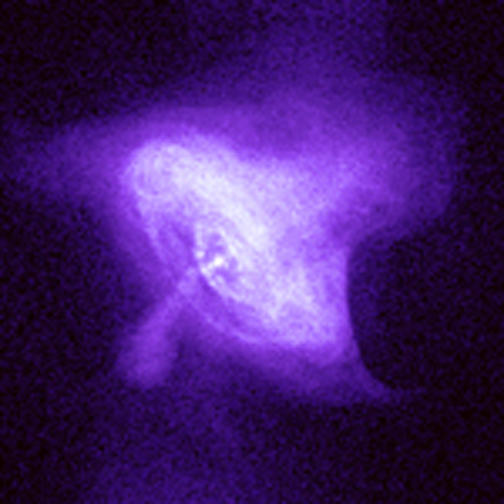
\includegraphics[width=0.5\columnwidth]{0052_xray_lg.jpg}
\end{center}
\caption{The central region of the Crab Nebula as seen by the Chandra
  X-ray Observatory. Credit: NASA/CXC/SAO)}
\label{fig:crab-xray}
\end{figure}

\begin{enumerate}
\item {\bf Hot cloud:} 

  X-ray photons are produced in a cloud of radius $R$ at the uniform
  rate $\Gamma$ (photons per unit volume per unit time) as in
  Fig.~\ref{fig:crab-xray}.  The cloud is a distance $d$ away.
  Assume that the cloud is optically thin.  A detector at Earth has an
  angular acceptance beam of half-angle $\Delta \theta$ and an
  effective area $\Delta A$.
\begin{enumerate}
\item If the cloud is fully resolved by the detector what is the
  observed intensity of the radiation as a function of position?
\item If the cloud is fully unresolved, what is the average intensity
  when the source is in the detector?
\end{enumerate}
\item {\bf Brightness Temperature:}
\index{temperature!brightness}

From the equation of radiative transfer derive an equation describing
how the brightness temperature changes as radiation passes through a
thermally emitting gas.  You may neglect scattering and assume that
the emission is in the Rayleigh-Jeans limit.  Solve this equation to
give the brightness temperature as a function of optical depth,
assuming that the gas has a constant temperature. 

\item {\bf Neutrino Blackbody:} 
\index{radiation!blackbody!neutrino}

Only one or no neutrinos can occupy a single state.  Calculate the
spectrum of the neutrino field in thermal equilibrium (neglect the
mass of the neutrino).  Neutrinos like photons have two polarization
states.  What is the ratio of the Stefan-Boltzmann constant for
neutrinos to that of photons?

\item {\bf Blackbody radiation:}
\begin{enumerate}
\item Show that if stimulated emission is neglected, leaving only two
  Einstein coefficients, an appropriate relation between the
  coefficients will be consistent with thermal equilibrium between an
  atom and a radiation field with a Wien spectrum, {\em i.e.} $B_\nu
  \propto \nu^3 \exp[-h\nu/(kT)]$.
\item Derive the relationships between the Einstein coefficients of an
  atom in equilibrium with a neutrino field.  
\end{enumerate}
\item {\bf Surface Emission from the Crab Pulsar:}  The neutron star
  that powers the Crab Pulsar can be assumed to have a mass of
  $1.4\mathrm{M}_\odot$ and a radius of 10~km with constant internal
  density and an effective temperature of $10^6$~K.  The frequency of
  the Crab Pulsar is 30~Hz and its period increases by 38 ns each
  day.  Compare the power from the surface emission to the power
  lost as the neutron star spins down.  The total power of the Crab
  Nebulae is about 75,000 times that of the Sun.  What is the likely
  source of this power?
\item {\bf Power-law Atmosphere:}  Assume the following
\begin{itemize}
\item The Rosseland mean
  opacity is related to the density and temperature of the gas through
  a power-law relationship,
$$
\kappa_R = \kappa_0 \rho^{\alpha} T^{\beta};
$$
\item The pressure of the gas is given by the ideal gas law;
\item The gas is in hydrostatic equilibrium so $p=g\Sigma$ where
$g$ is the surface gravity; and
\item The gas is in radiative equilibrium with the radiation field so 
the flux is constant with respect to $z$ or $\Sigma$.
\end{itemize}
Calculate the temperature of the gas as a function of $\Sigma$.
Assuming that the Crab pulsar has a surface or effective temperature
of $10^6$~K, what is the temperature at a density of
$10^7$~g/cm$^{-3}$ in the interior of the neutron star?  You may
assume $\alpha=2$, $g=10^{14}$ cm/s$^2$ and
$$
\kappa_R = 3.68 \times 10^{22} g_{ff}(1 - Z)(1 + X) \rho T^{-7/2} {\rm cm^2 g^{-1}}.
$$
where $\rho$ is given in g/cm$^{-3}$ and $T$ is given in Kelvin.

\item {\bf Goggles:}
\index{goggles}
Calculate from thermodynamic principles how much objects are magnified
or demagnified while viewed through goggles underwater.

\item {\bf Intensity and index of refraction: }
How does the intensity of light travelling along a ray change when the
light enters a material with a different index of refraction?
\begin{enumerate}
\item Solve this problem using geometry.
\item Solve this problem using thermodynamic principles alone.
N.B. The wavenumber of a photon of a given frequency is proportional
to the index of refraction.
\end{enumerate}
\end{enumerate}

 	
%%% Local Variables:
%%% TeX-master: "book"
%%% End: